\documentclass[12pt, a4paper]{extreport}
\usepackage[utf8]{inputenc}
\usepackage{graphicx}
\usepackage{titlesec, color, blindtext}
\usepackage[
    style=ieee
]{biblatex}
\usepackage[toc]{appendix} % use [page] to include appendix title page

\addbibresource{references.bib}
\setlength{\parindent}{4em}
\setlength{\parskip}{1em}
\definecolor{gray75}{gray}{0.75}
\newcommand{\hsp}{\hspace{10pt}}
\titleformat{\chapter}[display]{\Huge\bfseries}{Chapter \thechapter}{0.3em}{\LARGE\bfseries}
\titlespacing*{\chapter}{0cm}{-\topskip}{0pt}[0pt]
\titlespacing*{\section}{0cm}{0cm}{0pt}[0pt]

\title{Using Containers to Isolate Remote Code Execution for an Online Development Environment}
\author{
    Joseph Fazzino\\
    24026478\\
    [4cm]{Supervisor: Dr. Hong Wei}
}
\date{29\textsuperscript{th} April 2019}


\begin{document}

\maketitle

\tableofcontents
% --------------------------------------------------
% Preamble
% --------------------------------------------------
\pagebreak

% --------------------------------------------------
% Abstract
% --------------------------------------------------
\section{Abstract}
250 - 300 words

outline aims, methods, implementation, achievements, and conclusions
\pagebreak




\pagebreak

% --------------------------------------------------
% Acknowledgements
% --------------------------------------------------
\section{Acknowledgements}
I'd like to acknowledge Dr. Hong Wei for being my project supervisor. Dan Justin and Dr. Martine Magnan for their continued support through the early stages of my career. Suhail Parmar for contributing to my caffeine levels and providing help with Docker and UNIX. Dan Davis and Max Denning for helping me brainstorm the idea for the project and enduring me talking about frontend for the past year. And finally, my parents, Paul and Joanna Fazzino for being unwaveringly supportive and great role models.
\pagebreak


\pagebreak

% --------------------------------------------------
% Glossary
% --------------------------------------------------
\section{Glossary of Terms and Abbreviations}
The following is a list of abbreviations that are commonly used in this document:

API - Application Platform Interface

RTC - Real-Time Communication

REPL - Read-Evaluate-Print-Loop

HCI - Human Computer Interaction

UX - User Experience

DX - Developer Experience

UI - User Interface

JS - JavaScript

OS - Operating System

PaaS - Platform as a Service

VM - Virtual Machine

VPN - Virtual Private Network
\pagebreak

% --------------------------------------------------
% Table of Contents & Glossary
% --------------------------------------------------



% --------------------------------------------------
% Thesis
% --------------------------------------------------
% --------------------------------------------------
% Introduction
% --------------------------------------------------
\chapter{Introduction}

As computers have become more pervasive, programming has become a skill that has graduated past being something that only people who work in laboratories need to concern themselves with, to a skill that has become highly desirable commercially and is starting to be taught in the regular curriculum to children studying at a primary school level \cite{schools}. This has created a demand for beginner friendly programming tools and environments, this project is proposing to provide a tool to fill this niche by creating an online environment where people can get started with basic programming concepts without having to trawl through documentation and technical detail about how to get running with one of the popular languages/tools available.

This project is attempting to lower the barrier to entry for anyone with an internet connection to be able to get started programming with as little overhead as possible with an environment which is personal.

\pagebreak


% --------------------------------------------------
% Problem Definition / Technical Specification
% --------------------------------------------------
\chapter{Problem Articulation\\ \& Technical Specification} \label{chapter:probart}
% Here you must provide a detailed description of the problem being addressed. 
% This should include a problem statement and description of the context/environment of the problem 
% along with the key stakeholders and their concerns. The problem statement should be succinct 
% and should establish the criteria  by  which  the  problem  would  be  validated  and  accepted  
% as  being  adequately  solved  (i.e. acceptance requirements). 
% A technical specification may be developed against which a range of possible solutions, 
% including the one you implement, can be considered later in your report. 
% Again the PID content should help you when composing this section. You would include an 
% analysis of the situation-as-is. In some cases this may be very simple. 
% In others with socio-technical system contexts it could be complex and require system / architecture  / environment representations 
% (e.g. in algorithms, mathematical models, UML models, XML, ArchiMate models or other means 
% suitable to your domain). You would also include a vision of the situation-to-be where  the  
% problem  is  adequately  solved.  Again  this  might  require  complex  representations.  
% The situation-to-be and its representation should help you when composing the Discussion section.
\section{Context} \label{section:probart-context}
As computers have become more pervasive, coding has become a skill that has graduated past being something that only people who work in laboratories need to concern themselves with, to a skill that has become highly desirable commercially and is starting to be taught in the regular curriculum to children studying at a primary level education\cite{schools}. This new demand for beginner friendly coding tools lends itself nicely to the promise of an online based environment where people can get started with basic coding concepts without having to trawl through documentation and technical detail about how to get running with one of the popular languages/tools available. This has led to an explosion of popularity for web applications such as \texttt{codecademy.com} which offer pre-made, executable exercises for a number of languages. A similar platform \texttt{repl.it} offers a more open and free-form experience and attempts to recreate the environment a developer may have on their machine through the web browser along with online compilation.

\section{Problem Statement} \label{section:probart-probstate}
A common pattern with the current platforms that exist is that they provide a strict sandbox within the confines of a predetermined configuration that the user selects, for example, in \texttt{codecademy} and \texttt{repl.it} you're stuck in the environment you pick when you start desired tool. An argument can be made that this makes a new developers life easier as they don't have to consider the more nuanced parts of the file system or learn any sort of terminal commands. However, it seems as though there would be value in a system that can provide both the ease of use that current existing solutions offer and also the freedom to explore a full environment with an array of tools preconfigured that encourage exploration without compromising the security and integrity of the underlying system.

\section{Technical Specification} \label{section:probart-techspec}
Based on the problem statement the potential scope for the project is very broad, there are companies and teams of developers that have the sole goal of making sure their online environments are providing users with as smooth an experience as they would expect if they had installed the tools locally.

This project will focus on the essential functionality required to behave as an online development environment while supporting a good variety of languages and offering a space which encourages exploration into different coding concepts.

With the above in mind the enumerated objectives of this project are: 
\begin{enumerate}
    \item Create a platform where users can write/execute code
    \item Give every user their own personal environment
    \item Eliminate the need for locally installed tooling
    \item Provide a system that encourages exploration into the world of development
\end{enumerate}

\subsection{Writing and Executing Code}
As an essential requirement for the development experience, the ability to edit and execute code is crucial to satisfy the overarching objective of creating an online environment. The execution of code presents a significant technical challenge however as the only code execution that can be done remotely is on a web browser which must be able to execute HTML, CSS and JavaScript. Mobile applications developed for iOS and Android are not capable of executing code.

\subsubsection{Functional Requirements}
\begin{itemize}
    \item Code will be able to be typed using the platform
    \item Code will be able to be saved
    \item Code will be able to be read from the platform
    \item Code will be able to be executed
\end{itemize}
\subsubsection{Non-Functional Requirements}
\begin{itemize}
    \item A good variety of languages will be supported
    \item The basic features of a code editor will be available (i.e. syntax highlighting)
    \item Code that is executing will not stall the platform
\end{itemize}

\subsection{Personal Environments}
The need for the space that the user occupies to feel personal is a vital element to local development environment and therefore must be well implemented for an online equivalent.

\subsubsection{Functional Requirements}
\begin{itemize}
    \item A personal environment will be allocated to every user
\end{itemize}
\subsubsection{Non-Functional Requirements}
\begin{itemize}
    \item The personal environments will be isolated from the rest of the system
    \item The personal environments will be isolated from each other
    \item The personal environments will perform well and be responsive to user input
    \item If a personal environment fails then it will be restarted
\end{itemize}

\subsection{Local Tooling Replacement}
Tooling has been through some big changes both in web browsers and locally. Web browsers have got to the point where they are so powerful that some of the most popular desktop software is being powered by them\cite{carlo}. It is important to provide tools that will help those new to development, while also offering experience in tools that are of a high quality.

\subsubsection{Functional Requirements}
\begin{itemize}
    \item High quality tools will be available to the user
    \item Industry standard tools will be available to the user
    \item The system will eliminate the need for local tooling
\end{itemize}
\subsubsection{Non-Functional Requirements}
\begin{itemize}
    \item Popular tools will be researched and considered before being added to the system
    \item Tools will be standardised across the system
    \item Tools will be customisable to the users needs
    \item Tools will behave in a responsive manner
\end{itemize}

\subsection{Encourage Exploration into Development}
Lowering the barrier to entry through the requirements stated above will inherently make it easier to explore development but more steps can be taken in order to engage users with the system such as allowing them to create short coding exercises that can be shared with friends or on social media.

\subsubsection{Functional Requirements}
\begin{itemize}
    \item Implement exercises for users to do
    \item Allow creation of exercises by users
\end{itemize}
\subsubsection{Non-Functional Requirements}
\begin{itemize}
    \item Allow any exercise to be shared
    \item Assign difficulty level to exercises
    \item Provide an open area for the user to explore their personal environment
\end{itemize}

\section{Stakeholders} \label{section:probart-stake}
This project has a number of relevant stakeholders with various degrees of interest in the outcomes. All of them will be considered during the construction of the system.

\subsubsection{The Developer - Joseph Fazzino}
The developer of the system is responsible for making 100\% of the the technical decisions and is responsible for delivering a fully functioning system adhering to the technical specification found in  Section \ref{section:probart-techspec} of this report.

\subsubsection{Project Supervisor - Dr. Hong Wei}
The supervisor of this project is overseeing the development and design process that is being undertaken. 

They provide guidance when it comes to essential functionality and ways that technical requirements can be implemented.

\subsubsection{User - Beginner Level Developer}
Those new to development will not have experience with the terminology and syntax that exists in programming and wider computer science. They may have an understanding of basic coding concepts taught to them during formal education.

The beginner user should be able to use the system in order to become more familiar with generic programming concepts. The exercises available through the system will likely be the area they spend the most time.

\subsubsection{User - Intermediate Level Developer}
A user more familiar with the general work flow of a developer will be able to understand certain levels of nuance of how a system might be implemented and consider how they may solve certain problems.

This kind of user would benefit more from the ability to have a playground to explore the system in so they can understand the functionality that it provides and maybe try to explore the extent to which it works.

\subsubsection{User - Experienced Level Developer}
This user will have successfully developed systems with a high level of complexity and will most likely have specialised knowledge in a certain domain/environment.

This type of developer will be difficult to convince the benefits of an online working environment when they undoubtedly have a solution that works well for them locally.

\section{Constraints} \label{section:probart-constraints}
Some constraints on the development of the project exist.

\begin{itemize}
    \item Permanent deployment - as the system is likely to be complex, deploying it will be costly and time consuming. Test deployment will be done to experiment with configuration settings in the system but a permanent live deployment will not be.
    \item Computer resource availability - the system will be constrained performance wise by the resources available during development meaning that any stress tests are not representative of a deployed system
    \item Significant testing base - as the system will not be deployed it will be difficult to adequately test the system in the manner which it would be used by end user. A different method of testing will have to be explored.
\end{itemize}

\section{Assumptions} \label{section:probart-assumptions}
A number of assumptions must be made to reasonably meet the technical requirements.

\begin{itemize}
    \item The users will have a reliable internet connection
    \item The users will have the necessary software/hardware configuration in order to access the system (e.g. a modern web browser)
\end{itemize}

% --------------------------------------------------
% Literature Review
% --------------------------------------------------
% The literature review is an essential component of your project report. You should discuss the existing literature that is relevant to your project with full and proper referencing. You should aim to refer to a range of material including academic papers, text books, articles and existing product descriptions. It should be clear to the reader why the literature you identify is relevant and how you have incorporated the learnings from your review into your project. For example, you may have made a number of project 
% Page 4 of 5 decisions based on your review of the literature and these decisions should be described. The literature review should also lead to the creation of a number of possible solutions to your problem articulation and technical specification

\chapter{Literature Review} \label{lit}

This chapter examines various literature around relevant subjects to the project objectives stated in Section \ref{section:probart-techspec}. It looks at the various methods of \textbf{Real-Time Communication} that exist in order to create an environment where feedback is fast and frequent \textit{(Section \ref{lit-rtc})}. It examines some \textbf{existing systems} that are providing some of the features listed out and critically examines the positives and negatives of some of the technical choices that are apparent in these systems \textit{(Section \ref{lit-ode})}. It also analyses some of the modern advances in \textbf{Virtualisation} technology along with how the advent of \textbf{Containers} have changed the landscape of PaaS services and virtual environments in general \textit{(Section \ref{lit-containers})}. It concludes by looking at the state of the art in \textbf{frontend} \textit{(Section \ref{lit-frontend})} and \textbf{backend} \textit{(Section \ref{lit-backend})} technologies that can be used to create a modern web application. 

\section{Real-Time Communication} \label{lit-rtc}

Real-Time Communication is an important research topic for this project as in order to create an environment for users that feels as close to a local experience as possible, the requirement for fast feedback is essential.

An experiment was done in 2012 discussing the performance of different RTC methods by Professors at the University of New Brunswick \cite{websocket}. This experiment compared the different standard HTTP methods of implementing Real-Time Communication compared to the new (at the time) technology of WebSockets which are designed to create a fully duplexed bidirectional data-flow.

\textbf{HTTP polling} is an attempt to solve the real-time issue by repeatedly making a request to a web server at a pre determined time interval to check to see if there are any messages waiting to be read.  \textbf{HTTP long-polling} is another solution that uses the HTTP protocol but reduces the number of wasteful requests by having the server intelligently not respond to the request if there is no information available and hang until a timeout or information becomes available. Both of these solutions are inadaquate for a responsive system however because the HTTP protocol is still built on top of a system not designed for real-time, fully duplexed communication channel. HTTP relies on a standard 'Request-Response' model which is only half duplex so polling was only a solution that worked for systems that were reliably sending data at a steady rate such as sensors that are being queried for an API.

A modern solution to this is the \textbf{WebSocket} protocol proposed in RFC 6455 \cite{wsrfc} which aims to reduce latency by a factor of 3 compared to HTTP in the real-time communication aspect. It is a fully duplexed, bidirectional communication channel that provides an efficient method of communicating between several different clients using a persistent connection between the client and the server. A client may connect to a websocket endpoint on the server, send messages to it, and the server may broadcast messages back to just that client or to every client connected. Due to this behaviour it is very popular for creating text based chat communication systems.

WebSockets work by utilising a persistent TCP connection where messages can be sent back and forth without there having to be a new connection made every time. This behaviour is possible in HTTP since HTTP 1.1 however, WebSockets do not adhere to the standard, 'Request-Response' cycle that a HTTP request utilises. Any client connected to the socket is capable of broadcasting a message at any time. HTTP persistent connections also still suffer from latency due to the effort the protocol makes to control congestion \cite{httpvsws}. WebSockets take the concept further by making it simple to embed data with each request in the form of a string in the form of a JSON schema. This makes it ideal for the transfer of small chunks of text where only text is the required form of the response. WebSockets are not appropriate for downloading resources or assets such as images.

Another new approach of RTC on the web has been developed by Google in collaboration with other browser vendors called \textbf{WebRTC} \cite{webrtc}. This technology is focused on streaming audio and video between different clients on the web. This new technology is aiming to be the replacement for the browser plugins that were necessary in order to use P2P video/voice chat software such as \textit{Skype, Facebook Messenger, Google Hangouts, etcetra} \cite{webrtc}. WebRTC is more appropriate for applications that need a streaming based connection as it's latency is even lower than WebSockets due to it utilising the UDP protocol which has much less overhead compared to the TCP based connection of WebSockets \cite{udpvstcp}. WebRTC would not be appropriate for the use case of WebSockets as when transferring informational data between clients, such as a chat application, it is important to make sure that the data is being received in the correct order whereas UDP is less concerned so long as enough packets get transferred to create a stable audio/video connection.

\begin{figure}[h!]
    \centering
    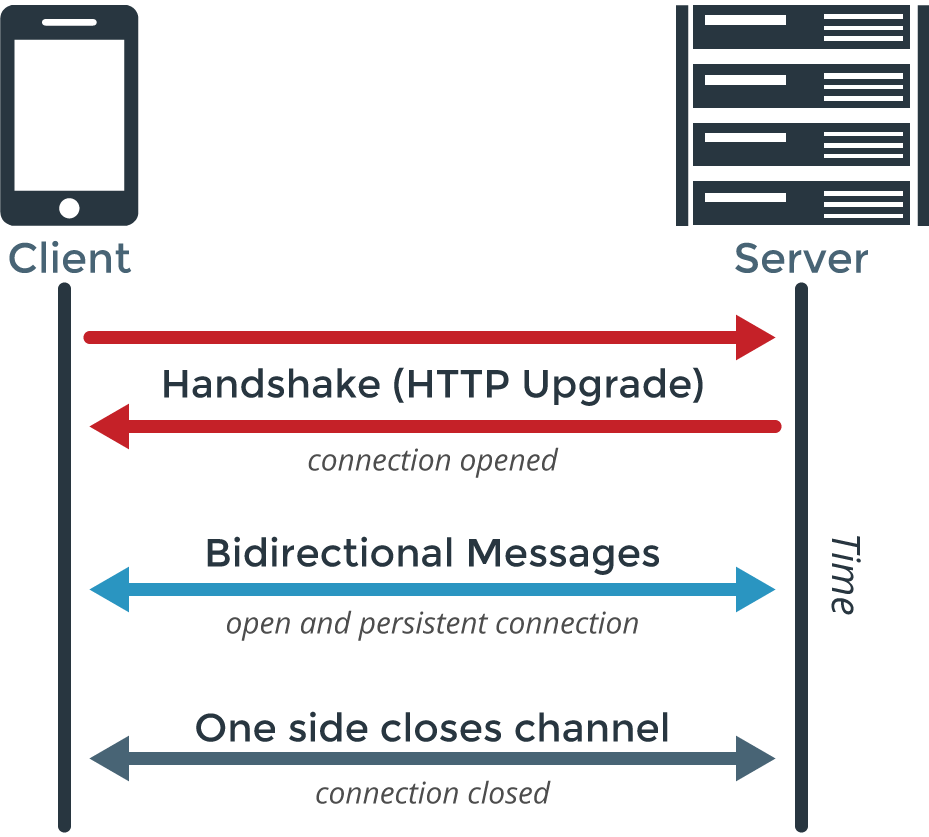
\includegraphics[scale=0.3]{res/WebSockets-Diagram.png}
    \caption{Illustration of WebSocket connection \cite{websocket-img}}
    \label{}
\end{figure}

\section{Online Developer Environments} \label{lit-ode}

A number of existing solutions providing online development environments exist and have been analysed for the purpose of this review.

\subsection{Repl.it}

Repl.it is very similar to the idea proposed in the Problem Statement (Section \ref{section:probart-probstate}) and a lot of the requirements lined out in Section \ref{section:probart-techspec}. It offers a huge array of Repl templates available for users to get started with many languages/frameworks very quickly. It also uses the Monaco Editor provided by Microsoft in order to provide a first class text editor experience.

Repl.it takes advantage of containers in order to gives users a full developer experience when visiting the system \cite{replit-containers}. The system also uses it's own container orchestration software in order to scale the instances available to users up and down depending on demand and predicted demand.

Every code result that is available to be viewed/run is viewable through a special .repl.run subdomain. This includes long running processes like web servers which are able to be hosted from these subdomains and be always accessible. This means you could create several repls which all connect to each other like a full system.

Technically the system is very impressive, something that the system doesn't recreate quite as smoothly as a local environment would is a small amount of latency between a key being pressed and the corresponding value appearing in the REPL itself.

The system also seems to remove all previously typed entries of the REPL on every press of the \textit{Run} button. This suggests that it is giving you a new REPL instance on every execution which isn't how a local environment works.

From a HCI point of view the website feels very smooth to use and is not frustrating to use other than the latency noted when typing directly into the running container via the REPL.

Repl.it is clearly very focused on the objective of replacing local development environments and does a good job of fulfilling that need.

\subsection{Codecademy}
Codecademy is a educational focused online environment designed to teach users how to code. Ranging in topics from beginning web development to a course on the IBM Watson API. It is a more directed experience than Repl.it as users are performing tasks for exercises but they are typing code into a similar environment, the code is executed and the result is displayed to the user.

Codecademy does not allow access directly to the REPL but if code is entered into the editor which allows for user input such as the \texttt{input()} function in Python. Then it interprets the input correctly.

The Codecademy web application is clearly a very complicated system and it shows by how unresponsive it feels when navigating from page to page. The page does a full refresh even though there are elements which do not change on the screen page to page. This leads to a frustrating wait looking a blank screen between page loads.

It is clear that Codecademy is a focused environment to encourage new developers to get into development by offering an easy to start environment and heavily directed experience. It is not concerned with the idea of replacing local development environments so much as making sure that it's not something beginners should need to think of when wanted to get to know a new tool.

\subsection{Glitch}
Glitch is a web application that is focused on trying to cultivate a social coding community that encourages developers to help each other out and build mini applications with JavaScript and Node.js. It provides an online coding environment that uses containers to isolate the users runtime.

Glitch is clearly focused heavily on the social aspect as on the homepage they have a section dedicated to users asking for help so more experienced coders can help them achieve their goals with the applications they want to build. It also showcases user made projects on the homepage which can be \textit{Remixed} which is similar to forking a repository on GitHub for other users to modify.

In terms of design, the website has a very colourful friendly interface. A feature which is particularly notable is in each project editor there is an option to view \textit{Container Stats} where the CPU usage in \%, Memory usage in bytes and additional relevant information can be found. There is also guidelines on the technical restrictions for projects that are run in Glitch. 


\section{Virtual Machines and Containers} \label{lit-containers}

In order to provide as close to local experience as possible to the users of the system this project aims to create. A virtual environment for executing code and saving files is vital. Virtualisation technology is changing significantly due to the different Container solutions which attempt to promote a more disposable and lightweight type of virtual environment compared to their hypervisor powered counterparts.

\subsection{Virtual Machines}

Virtualisation is a technique in computing that, most commonly, is seen by users in the \textbf{Virtual Machine} (VM software. Virtual Machines are heavily utilised to provide virtual desktop environments on top of a users already existing desktop. The advantages of which are, a sandbox environment for potentially harmful operations, such as when penetration testers are trying to fingerprint a virus. The option of trying a different OS without needing to dedicate a partition of disk space to it or deal with a dual booting set up is another user facing benefit of virtual machines.

In the enterprise world, Virtual Machines are being used to host their customers applications in a full Platform-as-a-Service (PaaS) solution so customers no longer have to worry about hosting their own web servers or other online services.

The general way of interacting with fully virtualised environments is through a hypervisor which is a tool that is responsible for provisioning and monitoring Virtual Machines \cite{hypervisor}. The hypervisor allocates resources such as memory and CPU cores from the host machine that the VM is allowed to consume. When the VM is shut down these resources are freed and can be used by the host system once again. The hypervisor also allows the VM to use a different base operating system than the one that is on the host machine as it provides a whole \textit{Guest OS}.

\subsection{Containers}

Containers are a much lighter virtualisation method than  Virtual Machines despite the functionality being similar. They achieve this as they are much closer to the systems 'bare metal' as any commands that are executed through a container are running on the host's hardware. This means that there is no need for a hypervisor as containers have direct access to the system resources. Usage limits can be set in the configuration of container \textit{images}.

As Containers traditionally don't utilise a hypervisor the biggest difference between them is that the engine that powers the container provisioning software such as the \textit{Docker Engine} isn't able to virtualise an environment based on a different OS. This is more by design however as it is what gives containers their 'lightweight' quality as they aren't having to simulate a whole kernel. Not having a full kernel to set up however means that containers can start up significantly faster than a VM.

\begin{figure}[h!]
    \centering
    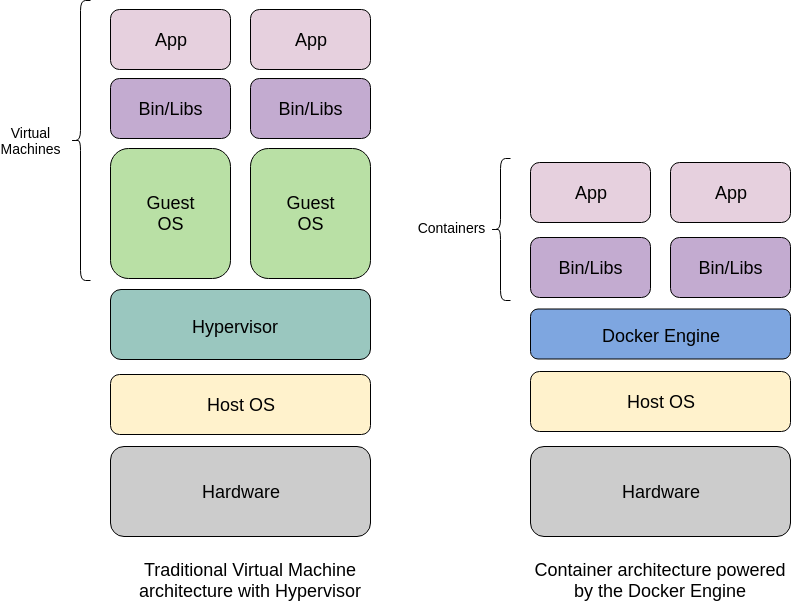
\includegraphics[scale=0.4]{res/Virtualisation.png}
    \caption{Architecture of Virtual Machines vs. Containers}
    \label{fig:architecture}
\end{figure}

Due to their performance benefits containers have become popular options for PaaS software. A paper was written comparing the benefits of a fully virtualised environment against a container based solution \cite{contsvsvirt}. It concluded that containers have an inherent advantage over VMs due to the performance benefits and the quick start up time of them. It also mentions that few PaaS vendors are using containers for their systems so far as they are too new of a technology. It is worth nothing that the report was published in 2014 however and since then uptake will have increased.
\pagebreak
\section{Container Providers}

As containers are a more modern innovation than hypervisors, recently there has been a wave of different technologies that attempt to make simple containers in varying ways.

\subsection{Linux Containers}

As briefly mentioned above, \textbf{Linux Containers} or \textbf{LXC} are the foundation of many container solutions. This is due to the fact that they offer a light kernel implementation which provides every container with some key features.

\begin{itemize}
    \item A unique Process ID for each container
    \item Isolates all resources for the container by using cgroups and namespaces
    \item Provides each container with it's own private IP address
    \item Isolates all files on the container from the Host by using chroot
\end{itemize}

%TODO: explain cgroups and namespaces
The features listed above are all features standard in the Linux kernel. \texttt{cgroups} \cite{cgroups-man} or control groups are a feature that is able to isolate and allocate resources from the machine to each individual process. 

\texttt{namespaces} \cite{namespaces-man} is another key feature of the kernel which LXC relies on in order to provide isolation to each container. The purpose of namespaces is to wrap a process or a group of processes in an isolated instance of the global resource, changes of global resources are to other processes that are a member of a namespace but aren't visible to other namespaces.

In terms of downsides the LXC implementation is heavily tied to the Linux OS which means that it is not possible to run it on a different OS such as Windows. There are also some security concerns for LXC as all the containers share the one host kernel.

\subsection{OpenVZ Containers}

OpenVZ makes use of a modified Linux kernel with it's own set of extensions. OpenVZ is able to manage physical and virtual servers with \textit{dynamic real-time partitioning}. It similarly offers better performance than a traditional hypervisor based system and utilises the cgroups and namespaces features of Linux to provide it's virtual environments.

On top of the advantages of LXC it also provides the following benefits.

\begin{itemize}
    \item \textbf{Container Lifecycle} remote management can be done of containers using an API to modify the status of a container in real-time. 
    \item \textbf{Container State} is able to create checkpoints during the container's lifecycle so that it may be recovered from that point should anything go wrong.
\end{itemize}

These mean that there is greater user access over the state of containers and that restoration points can be created to store users progress with a container.

\subsection{Docker}

The Docker process is a daemon which can provide and manage Linux Containers as \textit{images}. It uses LXC for the container implementation and then adds on top an image management system and a \textit{Union File System}.

Using the daemon, Docker manages to provide similar functionality as the OpenVZ containers in relation to lifecycle and state. The state of a container at any time can be saved to a new image which can then be reloaded by the daemon to that same point

Unlike OpenVZ, Docker can be run with the standard Linux kernel and therefore is more suited for PaaS software. It also has a thriving ecosystem of pre-made images which offer a huge array of different starting points and tools.


\section{Frontend Web Technologies} \label{lit-frontend}

The client side of web applications is based on three fundamental technologies, \texttt{HTML}, \texttt{CSS} and \texttt{JavaScript} which declare both the layout of the application and the functionality.

Web development has changed a lot since its inception, new technology has been released that gives developer greater flexibility in how they build their modern web apps. Since the creation of jQuery \cite{jquery} a number of JavaScript based frameworks/libraries have come about that try to solve some of the problems that are inherent to the web platform.

\subsection{React}

React is developed by Facebook and attempts to simplify the process of creating interactive UIs by providing a declarative way of writing UI code and encouraging the reuse of \textit{components} which are composed HTML elements with the ability to provide interaction through JavaScript.

The need for a library such as React comes from the difficulty involved with maintaining data synchronisation between what is displayed on the screen and variables that exist in the JavaScript code. React also offers a high amount of code reuse with its component architecture. 

React is able to use JavaScript functionality inline with HTML style layout syntax by providing it's own version of HTML called JSX.

React has a very strong community with over 80,000 packages listed on the npm package registry \cite{npm-search-react}.

\subsection{Vue.js}

Vue.js is a JavaScript Framework that offers a lot of the same functionality as React but offers it in a way that is more akin to the traditional way that web development is done. Where React blends the 3 key technologies of the web into a JavaScript focus. Vue.js maintains a separation of these concepts.

Vue.js offers more than React out of the box such as an official routing solution for single page applications, global state management and server side rendering.

Vue uses ordinary HTML as it's view templating however it is able to inject it's own directives and JavaScript functionality by making use of the popular handlebars syntax.

It has grown very quickly since it came out in 2014 and has just over 25,000 packages published on npm \cite{npm-search-vue}.

\section{Backend Technologies} \label{lit-backend}

There are numerous tools in use both professionally and recreationally to create web servers, databases, and other tools that a system might need to utilise. 

Traditionally, the backend of an application was written in a large framework such as \texttt{PHP} or \texttt{.NET}. In more recent times however, there has been a rise of lighter scripting languages such as \texttt{Python} or \texttt{JavaScript} which are powering infrastructure for some of the biggest technology companies in the world.

\subsection{Node.js}
Node.js \cite{nodejs} is a JavaScript runtime built on Google Chrome's V8 engine. As JavaScript is a single threaded language many thought it was unsuited to hosting backend applications due to the lack of concurrency available to it. Node.js uses the \texttt{libuv} C library \cite{libuv} in order to create an event loop which has the task of offloading external processes such as database calls and when a response come back the event loop can pass the result back to the JavaScript environment. This is how Node.js is made to be a viable option for hosting servers and running in a browser-less environment.

Node.js is in wide use in the industry with companies such as Netflix \cite{netflix-nodejs} which is a testament to how powerful it can be even at a huge scale like Netflix are using it. Node.js is also appropriate for use where the application is smaller in scale and perhaps only needs to interact with external processes and host some endpoints.

\subsection{.NET Core}

.NET Core \cite{.netcore} is a cross platform runtime developed by Microsoft which can be used to develop large scale web applications. 

.NET Core is able to provide a fullstack framework relying on Model-View-Controller architecture where the Models and Controllers are written in C\#, Visual Basic or F\# and the views are written in Microsoft's Razor syntax which is similar in idea to React or Vue's templating/JSX but uses C\# instead of JavaScript.

Being supported and created by Microsoft means that of course it's extremely useful for large scale applications that big companies will want to create. It is less well suited for smaller projects due to the MVC pattern which carries a lot of boilerplate. This can lead to writing a lot of code for simple controllers/views.

\pagebreak


% --------------------------------------------------
% Method
% --------------------------------------------------
\chapter{The Solution Approach}
\pagebreak


% --------------------------------------------------
% Implementation
% --------------------------------------------------
\chapter{Implementation}

% Here you describe the detailed design of your solution and the details of the actual implementation. It may be appropriate to discuss aspects of design or implementation that were particularly problematic and/or novel. This section may well be one of the largest in your report and the exact contents will be unique to your project and so there are no general guidelines. Use of several sub-sections here is appropriate.

This chapter focuses on the overall implementation of the system and walks through how the several separate systems interface together and interact in a way that provides the user with a positive experience.

\section{Backend}

The backend of the system is implemented in Node.js and provides the API that the frontend will interact with through REST requests and WebSocket messages. TypeScript \cite{typescript} is being used rather than plain JavaScript in order to provide support for static types and catch more errors during the build time compilation rather than during run time.

\subsection{Database}

The database is a straightforward MongoDB \cite{mongo} implementation with two collections, one for exercises and one for activities. An exercise can have many activities but activities can only belong to one exercise.

%TODO: Relational mapping?

For the Node server to be able to make database calls the MongoDB API must be queried against, this is done by using the \textbf{mongoose} package \cite{mongoose}.

\subsection{REST API}

To provide an API that a frontend can interact with to retrieve information from the database, a REST API is created with the Express framework \cite{express}. Creating an API endpoint with Express is a simple process that roughly follows the formula of:

\texttt{AppObject.RequestType("Endpoint", CallbackFunction)}

Where \textit{AppObject} is the variable representing the instance of the server. \textit{RequestType} is usually one of GET or POST. \textit{Endpoint} is a string representing the local path the handles the request and \textit{CallbackFunction} is the function that handles the request and sends the response.

so the code \texttt{app.get("/profile", callback)} is the function that would handle GET requests to the \textbf{/profile} endpoint. 

The only REST endpoints in the backend code are related to the exercises section of the system as those need to be stored in a global database. Most of the communication between the front and back is implemented through WebSocket connections.

\subsubsection{Get Exercise Endpoint}

The \textbf{/exercise} endpoint is a GET request that returns the related exercise in the database that corresponds with the ID that is sent along in the query string.

The callback function that deals with the request and sends a response is shown for this endpoint and it sends a response of 404 if it can't find the exercise based on the ID passed in the request and a 500 if there was an error with processing the request (such as if the database is down). Otherwise it will send a 200 and the exercise JSON object.

\begin{sexylisting}{Snippet for /exercise endpoint}
server.get("/exercise", (req: Request, res: Response) => {
    const { id } = req.query;

    Exercise.findById(id)
        .populate("activities")
        .exec()
        .then(exercise => {
            if (exercise) {
                res.send(exercise);
                return;
            }
            res.sendStatus(404);
        })
        .catch(err => {
            res.status(500).json(err);
        });
});
\end{sexylisting}

\subsubsection{Create Exercise Endpoint}

The \textbf{/create} endpoint is a POST request used when a user makes a new exercise. Here the request object is broken down to get the parameters sent with the request and is turned into objects that can be inserted into the database.

The response is the endpoint that the frontend can use to navigate to the page for the newly generated exercise.

\begin{sexylisting}{Snippet for /create endpoint}
server.post("/create", (req: Request, res: Response) => {
    /**
        Code to handle create request

        This is quite a lot of code refer to appendix %TODO:
    */
});
\end{sexylisting}

\subsection{Docker Integration}

For the backend to have the ability to create and link Docker containers to a user running the application on the frontend it needs to be able to interact with the \textit{Docker Socket}. Every machine with an installation of the Docker Engine has a Docker Socket which is what the Docker CLI uses when commands are run against it.

There is a popular package on NPM called \textbf{Dockerode} \cite{dockerode} which enables interaction with the Docker API via whatever socket/path is provided in it's configuration.

The following code snippet shows the instantiation of the Dockerode package using the local Docker socket and exports it for use in other files in the project's backend.

\begin{sexylisting}{Snippet to create Docker instance and point it to local Socket}    
import Docker = require("dockerode");
const SOCKET_PATH = "/var/run/docker.sock";
const options = { socketPath: SOCKET_PATH };
export default new Docker(options);
\end{sexylisting}

\subsubsection{Provisioning a User Allocated Container}

Creating a container for every user that connects to the system requires the concept of a \textit{basic image}. This image is a Dockerfile which specifies the defaults for all user's environments. The Dockerfile is responsible for configuring the environment so that it is secure and pre-installed with all the tools that the user might need.

The basic image, comes with the following software pre-installed: 

\begin{itemize}
    \item Alpine Linux Distro
    \item Bash
    \item Python3
    \item Node.js
    \item GCC
    \item Git
\end{itemize}

Alpine Linux is the distribution that the base image of the container which is based on Ubuntu. Bash is a very common shell which is a better default than the standard \textit{ash} or \textit{sh} which are the shells that come with the Alpine image. Bash is important for the code execution aspect of the system which is explained further in \textit{Executing Code - \ref{imp-execode}}. Python, Node and GCC are chosen as those are the 3 runtimes that are supported by the system. Git is installed so if the user writes something that they want to be able to save they can use Git through the command line.

% TODO: Ref the dockerfile in the appendix
Some additional configuration that is done in this Dockerfile is the creation of the user account that users of the system will be operating as while they're connected to the container. By default the Docker engine sets the user of a container as root but this is obviously not appropriate for a system where anyone can play with a container so a low permission user is created called \textit{damien} who has their own home folder and ownership of that folder but everything under the root directory is protected.

The JavaScript to create the container for the user is a simple function call referencing the Docker API variable.

\begin{sexylisting}{Snippet to create container with options}
const container = await docker.createContainer({
    Image: "basic",
    AttachStdin: true,
    AttachStdout: true,
    AttachStderr: true,
    Tty: true,
    Cmd: ["/bin/bash"],
    OpenStdin: true,
    StdinOnce: false,
    name
});
\end{sexylisting}

This tells the API to create a container using the image with the label "basic" which is what the Dockerfile described above has the label of. The various \texttt{AttachX} properties tell the container if they should allow other processes to attach to this containers Standard Input/Output/Error which, as this container is emulated on the front end is required to be \texttt{true}. Tty refers to an old way of referring to the interface for a terminal. Without this option set to true it won't display in a way that looks like a traditional command line environment. Cmd is the command that the container should run once it's been created, in this case it needs to run bash. OpenStdin allows standard input to the TTY. StdinOnce will close the STDIN connection if an attached user disconnects, this needs to be off for this system as going between an exercise and a container will detach in the way that satisfies this requirement and it needs to be able to reconnect to the STDIN. The name property is simply the labelled name of the container which is displayed to the user when they connect.

\subsubsection{Provisioning an Exercise Container}

Provisioning the exercise container is more or less the same as the user's allocated container but it has to pause the allocated container so that resources aren't being wasted and then create the container for the exercise.

Exercise containers are created when a user enters an exercise and are destroyed when a user leaves the exercise. The are created the same way with the same configuration as the allocated containers however the image they are based from is the simplest REPL image that exists that relates to the runtime that the exercise is for.

\subsubsection{Executing Code} \label{imp-execode}

Getting code from the server to inside a file on the container and then executing is a fundamental requirement of this project and is achieved by taking advantage of Bash which is configured to come on every container created by the system.

The execute command in Docker (exec) is only capable of running a single command with arguments. In Bash however there is a way of chaining commands as arguments using the \textbf{-c} option. A JavaScript function called \texttt{getCodeSaveCommand} creates the command that the Docker execute command can run in order to save the file.

\begin{sexylisting}{Snippet to create command to save code to container}
export function getCodeSaveCommand(filename, code) {
    let cmd = ["/bin/bash", "-c"];

    code = code.replace(/`/g, "\\`");

    cmd.push(`echo "${code}" > ${filename}`);

    return cmd;
}
\end{sexylisting}

This snippet will add an escape character in front of all double quotes so that the double quotes don't finish the \texttt{bash -c} command and add command that saves the code to the specified file to the cmd array. This array is what the CMD option accepts. 

After the file has been saved successfully a message is sent to the client confirming the save and the client sends an attach request for the code execution so that the STDIN and STDOUT can be attached to the terminal emulator.

The execute command to run the code is more straight forward than the command to save it to a file.

\begin{sexylisting}{Snippet for creating the code execution command for the container}
export function getCodeExecutionCommand(filename, repl) {
    let cmd = ["/bin/bash", "-c"];
    
    if (repl === Repl.C) {
        return cmd.concat(
            `gcc ${filename} && ./a.out && rm a.out`
        );
    } else {
        return cmd.concat(
            `${repl} ${filename}`
        );
    }
}
\end{sexylisting}

This snippet works along the same lines as the previous however more steps are involved for the C compilation step as an output file is generated which has to be executed.

\subsection{WebSockets}

As mentioned in the Solution Approach (Section \ref{solapp-rtc}) the standard WebSocket client that is available as a browser API and on the backend a middleware package \texttt{express-ws} \cite{expressws} is being used to allow connections to the server using the WebSocket protocol.

\subsubsection{Endpoint Configuration}

For the server to be able to create a WebSocket connection with clients and endpoint must be created that accepts the WebSocket protocol. 

\begin{sexylisting}{Snippet showing setup of WebSocket Endpoint}
    server.ws("/", (ws: WebSocket) => {
        console.log("Connection Made");
        startBasicContainer(ws)
        {...}
    }
\end{sexylisting}

The snippet above shows that a WebSocket connection can be made to the root endpoint of the server and once the connection is made it is logged to the console and the function to create the basic user allocated container is called.

\subsubsection{Message Structure}

WebSockets are only capable of sending strings of text in their messages however, as JSON is a way of representing objects through strings a template message guide can be created.

\begin{sexylisting}{Snippet showing WS message}
    const message = {
        type: MessageTypes.CONTAINER_STOP,
        data: { id }
    };

    socket.send(JSON.stringify(message));
\end{sexylisting}

This snippet shows that an example message which is a JSON object with two properties \texttt{type}, which represents the type of the message being sent, and \texttt{data} which is an object itself which contains any relevant information that might be useful for the other end of the socket. In this case the type of the message is a flag to stop a running container and the data is the ID of the container. This is sent after being stringify-ed by the built in JSON object.

\subsubsection{Message Types}

As can be seen above each message has a type. These types are processed through a \texttt{switch statement} which inspects the type, extracts the parameters from the \texttt{data} property and makes a function call.

\begin{sexylisting}{Snippet showing how the messages are processed by the backend}
    const { type, data } = JSON.parse(msg);
    switch (type) {
        case "Container.Pause":
            // Used when focus is lost from tab
            console.log("Pausing container");
            stopContainer(ws, data.id);
            break;
        case "Container.Resume":
            // Used when focus is resumed via tab
            console.log("Resuming container");
            resumeContainer(ws, data.id);
            break;
        {...}
\end{sexylisting}

The first thing that is done when the message is received is, as the message is a string, it is parsed into JavaScript objects and the \texttt{type} and \texttt{data} properties are extracted. The \texttt{type} is switched against and based on what the value of it is. A string is logged to the console showing what action the server is performing and a function is called which will always pass the WebSocket object (so the server can reply) and then passes any relevant data that is required by that function. 

\subsubsection{WebSocket Streams}

Streams is a concept in programming which quite directly means a \textit{stream of data}. Streams are used most often to act on a huge amount of data in a more performance focused way. Streams of events are the types of streams that are used in this project however as the Docker containers are able to stream their STDIN and STDOUT. Using the Node.js Stream API it is possible to \texttt{pipe()} these streams over WebSockets.

The package \texttt{websocket-stream} is used in the server to enable the streams to be piped over the WebSocket connection.

\begin{sexylisting}{Snippet showing endpoint which connects the container stream to the WebSocket}
server.ws("/connect", (ws: WebSocket, req: Request) => {
    const stream = websocketStream(ws, { binary: true });
    console.log("Trying to connect streams");

    attachSocketToContainer(
        stream,
        req.query.id,
        req.query.bidirectional,
        req.query.logs
    );
});
\end{sexylisting}

This snippet shows that a WebSocket connection can be opened to the \texttt{/connect} endpoint of the server where a stream will be created from the WebSocket. When the connection is made a function is called to attach the WebSocket stream to the container stream and it passes the stream created by the websocket-stream package, the id of the container to attach the stream to, whether the stream is bidirectional (allows STDIN and STDOUT) and if the previous logs from the container should be allowed.

Streams are a core concept in Node.js so passing one stream to another is simple.

\begin{sexylisting}{Snippet showing the attachment of the container stream to the WebSocket stream}
container.attach(
    {
        stream: true,
        stdout: true,
        stderr: true,
        stdin: isBidirectional,
        logs: showLogs
    },
    function(err: Error, stream) {
        {Error Handling here...}
        console.log("Stream Connection Established!");
        if (isBidirectional) {
            stream.pipe(wss);
            wss.pipe(stream);
        } else {
            stream.pipe(wss);
        }
    }
);
\end{sexylisting}

The snippet above is showing the Docker API making a call to attach to the running container which was calculated based off the ID passed to the function. The options show that the \texttt{stream} option is set to true, the \texttt{stdin} option is dependent on if the stream is set to be bidirectional or not and the \texttt{logs} are also determined by the parameter passed from the query string.

The callback function does error handling and then will pipe the container stream to the WebSocket stream. If bidirectional flow is enabled, it will also pipe the WebSocket stream to the container. 


\section{Frontend}

\subsection{WebSockets}

\subsection{Home Page}

\subsection{Sandbox Page}

\subsection{Exercises Page}

\subsection{Exercise Page}

\section{Tool Suite}

\subsection{Ahab}

\pagebreak


% --------------------------------------------------
% Testing and Validation
% --------------------------------------------------
\chapter{Testing: Verification and Validation}

% Here you explain your approach to testing and show your results. Testing should be a directed process and so there should be some discussion of why you have done the tests you have and why they are appropriate to the validation of your problem solution. You should also consider the limits to your presented verification and validation.

As this project has a lot of moving parts, testing is a necessary requirement to ensure how well the implementted system matches the objectives stated in Chapter \ref{chapter:probart} and the Project Initiation Document have been met and how robust the system is.

Testing of the actual code that composes the system was done with the Jest testing framework \cite{jest}.

\section{Usability Testing} \label{test:usability}

Usability testing is the process of making sure the features that have been implemented are all working by exercising them one by one and assessing their performance and quality.

\begin{table}[h]
    \centering
    \begin{tabulary}{\textwidth}{l|L}
        \hline
        \hline
        \textbf{Feature} & \textbf{Usability Summary}\\
        \hline
        \hline
        Monaco Text Editor & Feature works fully with syntax colouring, auto complete with JavaScript but not other languages\\

        Code Execution & Fully functioning in all areas that are applicable\\

        Terminal Emulator & Performs task well with input and output link issue with small level of latency where the messages are being buffered to only send every 10ms, leads to skipping some characters\\

        File browsing & Opening a file and saving to it works, issue where folders aren't displayed correctly\\

        Doing an exercise & Works, would be good for code validation to make sure the exercise output is correct but functionally works well\\

        Creating an exercise & Works well, currently C exercises can't be made due to the lack of C REPL available\\

        Sandbox Page & Would be good to have a run button like in the exercise page, also an issue with resizing windows going off the page\\

        Home Page & Would be nice if any code written in the windows was reloaded when the tab to switch language is pressed rather than just putting the default comment in.\\
    \end{tabulary}
    \caption{Usability testing of system}
\end{table}


% Code editing experience - v good

% Terminal emulator - some latency but not a deal breaker

% Run button on the sandbox page

% Nice having access to bash in the browser

% Expert mode idea for either the REPL or the bash Terminal

% Design - quite good

% Resizing windows - helpful

% Actually validate exercise output

% Error boundaries, react

% Error on homepage for when syntax is invalid etc

\section{Compatibility} \label{test:compat}

Although web applications don't have to be concerned about the computer system that the browser is relying on, several browsers use different engines and processors in order to render DOM elements to the screen. This means it's good practice to ensure the web application being developed is functional on the most different popular browsers.

\begin{table}[h]
    \centering
    \begin{tabulary}{\textwidth}{l|L|c}
        \hline
        \hline
        \textbf{Browser} & \textbf{UI Compatibility} & \textbf{Functionality Compatibility} \\
        \hline
        \hline
        Google Chrome & Fully compatible & Fully compatible \\
        Mozilla Firefox & Mostly compatible, only noticeable glitch is the page gains padding when the Monaco auto-complete appears & Fully compatible \\
        Microsoft Edge & Partially compatible, strange squashing of nav bar component & Fully compatible \\
        Apple Safari & Mostly compatible, some scaling issues with text & Fully compatible \\
        Internet Explorer 11 & Not compatible, the web app uses CSS Grid for page layout which is not supported in IE 11 & Un-testable
    \end{tabulary}
    \caption{Compatibility test results}
\end{table}

It's worth noting that Google Chrome's engine, Chromium is now powering a canary build of Microsoft Edge and is already powering Opera. This means that websites that are compatible with Chrome will be equally compatible with these browsers.  

Internet Explorer 11, while having the second highest market share of browsers \cite{browser-stats} is still only 9.83\% with Firefox close behind at 9.62\%. Overall coverage of the application is 84.83\% of all browsers which is a significant volume of users.

Adding support for IE 11 is an option for the future however, considering Microsoft are pushing their Edge browser over IE it isn't a high priority. Most of the usage will be enterprise users which can't run the latest versions of OS's or web browsers due to security concerns or long update cycles.

This compatibility test did not test mobile devices as they aren't supported by the Monaco editor so for now a landing page is rendered saying that mobile support is coming.

\section{Code}

Testing code is a way of making sure that the end product that is created is robust to future changes. Code testing can come in many forms but this project has focused on \textbf{Unit Testing}.

\subsection{Unit Testing} \label{test:unit}

Unit testing is the method of testing a component of the system as though it is a completely isolated module. A benefit of this is that when writing unit tests themselves it can reveal that code that was previously thought to be modular is not. 

Testing complex functionality is a high priority when thinking about writing unit tests. The WebSocket receiver functionality of the front-end is a good nomination for a test suite as it has many different outputs depending on the WebSocket event received. It also opens up the idea of Test Driven Development because if a new feature is being developed that would involve a new WebSocket event to be received, the event can be mocked (shown in Snippet \ref{snip:socket-test}) and the expected output can be defined. From this starting point the test will fail and the functionality can be added to the \texttt{switch statement} so that the test passes.

\begin{sexylisting}[label=snip:socket-test]{Test for Receiving Container.Start Message}
const MOCK_STATE = {};

test('Container Start', () => {
    const MOCK_EVENT = makeEvent(
        MessageTypes.CONTAINER_START, {
            name: 'Tester',
            info: { Config: { Hostname: 'Tester' } }
        });

    expect(handleMessage(MOCK_EVENT, MOCK_STATE))
        .toMatchSnapshot();

    const TEMP_STATE = { containerName: '', id: '' };

    expect(handleMessage(MOCK_EVENT, TEMP_STATE))
        .toMatchSnapshot();
});
\end{sexylisting}

This test is checking to see if when a mock event is passed to the function that handles the message, the output is correct and matches the previous snapshot. If the output changes (because the function changes) then this test will fail.

The back-end of the application can be tested in a very similar way by mocking inputs and snapshotting outputs. Functions can be tested in a way that means they are robust to future change in the code-base so any changes that are unexpected will cause the test to fails.

\section{Performance} \label{test:perf}

Performance testing is making sure that the system is working in an acceptably fast way. Measuring the performance of the front end is done by using the built in Lighthouse tool in Google Chrome and for the back-end, as it is famously difficult to measure Docker performance \cite{docker-perf} the measuring will be done locally with the Docker CLI \texttt{docker stats} command which provides real time information on the consumption of the containers that are running.

\subsection{Lighthouse Audits} \label{test:perf-light}

Built into Google Chrome is a website auditing tool called \textit{Lighthouse} \cite{google-lighthouse} which can measure many different aspects of web applications such as their performance, search engine optimisation, accessibility, and best practices. 

\textbf{Performance} is focused on areas such as the first meaningful paint to the screen and how quickly the web page is able to be interacted with. 

\textbf{Search Engine Optimisation (SEO)} is simulating how well a web crawler can crawl through the page and generate a sitemap so the pages are visible on a search engine. 

\textbf{Accessibility} measures important aspects such as if screen readers can interpret the elements on the page and if any colours aren't contrasting enough for those hard of sight to interpret the difference between.

\textbf{Best Practices} compares the website against industry standard of how to create a good modern website. This is a slightly more abstract concept to measure than the other sections however it is something Google consider important enough to include in their auditing tool. 

\begin{figure}[h!]
    \centering
    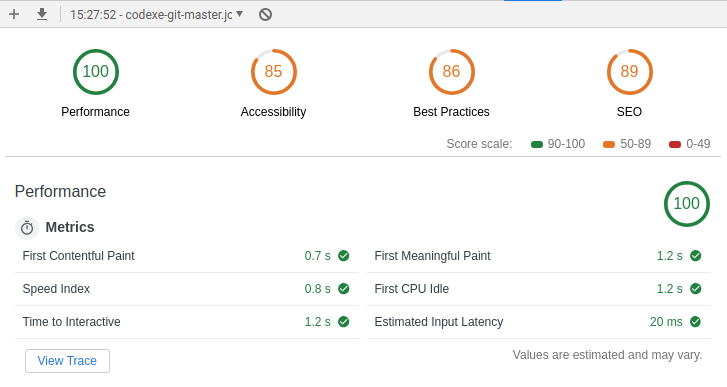
\includegraphics[scale=0.5]{res/lighthouse_audit_deployed.png}
    \caption{Lighthouse audit of deployed application}
    \label{deployed-lighthouse}
\end{figure}

The figure above shows some excellent results for the different measurements. Performance being 100 is particularly notable as most of Google's own products don't score that high. This performance result is due to how Next.js packages the application for deployment which converts all of the React layout code into regular HTML, CSS which is very fast to render. It also isolates each page into what they call a \textit{lambda} function which means that the pages aren't always running and instead will be loaded on demand. This means there's no resource wastage from a server running 24 hours a day. The different metrics are shown at the bottom of the figure with extremely fast response times. It is worth mentioning again that this is a deployed system and is not running locally or hosted on the same LAN.

The accessibility score is only 85 as the code editor's theme has the green of the comment which has low contrast compared to the dark background, there is also an issue in the bullet point list of site features as screen readers will announce the globe images when they shouldn't be noted. This can be fixed with an \texttt{aria-hidden} attribute on the element which will tell screen readers to ignore it. 

The best practices score is due to errors being logged in the console. As only the front-end is currently deployed, the WebSocket fails to connect which results in errors logged to the console. This will be resolved once the back-end of the application is deployed. 

The SEO score is due to there not being a meta description of the website in the \texttt{<head>} which is what provides search engines with their summary of the website. This is very easy to resolve. 

\subsection{Docker Stats} \label{test:perf-docker}

A number of tests were performed while visually observing the running of the \texttt{docker stats} command which provides real time usage on CPU, memory, I/O and more. It is worth noting before observing the results that while the usage can say 0\% that does not mean that 0\% of the CPU is being occupied by the container as there is a base level allocation of usage that, while may not be consumed, is still unavailable to other processes. This is mentioned in a report published discussing difficulties measuring Docker performance \cite{docker-perf}.

\begin{table}[h!]
    \centering
    \begin{tabulary}{\textwidth}{L|C|C}
        \hline
        \hline
        \textbf{Operation} & \textbf{CPU Usage (\%)} & \textbf{RAM Usage (MiB)}\\
        \hline
        \hline
        Server Started & Server Idling at 0.1 & Server Idling at 195.7\\
        
        Container Started & No change in server. New container 'Modi' idling at 0. & Server idling at 196.3. Modi idling at 1.234\\
        
        Counting to 50 million & Server jumps to 0.66. Modi peaks at 55. & No change in server. Modi peaked at 2.55. Modi idles higher post execution at 2.023\\
        
        Connecting the Terminal & Server jumps to 1. No change in Modi. & No changes in either container.\\
        
        Typing in the Terminal & Server peaks at 3.88. Modi peaks at 0.35. & No changes in either container.\\
        
        Opening a file & Server peaks at 0.7. Modi peaks at 4.3. & No changes in either container.\\
        
        Opening a Python Exercise & Server doesn't change. Modi pauses and idles at 0. Python container idles at 0. & No change in server memory use. Modi idles at 2.023 Python container idles at 5.625.\\
        
        Counting to 50 million in exercise & Server doesn't change. Python peaks at 50. & Server doesn't change. Python peaks at 8.\\
        
        Opening a new tab & Server behaves the same as opening container. New container idles with 0. & No change to server. Modi remains idling at 2.023. New container idles at 0.956.
    \end{tabulary}
    \caption{Results of \textit{docker stats} through different operations}
\end{table}

All tests were done 5 times and an average was taken. The specification of the machine that the testing was performed on is 3,500MHz CPU and 15,390MiB.

\section{Security} \label{test-sec}

% Pen testing

Security is a major concern with a system where users have the ability to not only execute code on a remote machine but also have access to the shell of a container that will be deployed to the same space as the entire back-end. Despite containers providing advantages speed/size wise over hypervisor powered virtual machines, from a security perspective there is a significant problem. The containers are running on the kernel of the machine that the container provisioning engine is running on so if a user is able to exploit a kernel bug, it means that they can break out of the container and start changing the shell of the machine hosting the entire system. This could be fatal if the attacker has malicious intent.

A lot of kernel exploits are only possible with root access so the first step to securing the containers is making sure that the user account that the users are logged into is not the normal Docker root user. This is briefly discussed in Section \ref{impl-alloc} with the Dockerfile that creates the \textit{damien} user which is what users are occupying while they're executing on the system. Inside this normal user account access to sensitive information is well secured, a lot of commands that can be used maliciously are locked and the ability to install software (like cracking tools and fingerprinting tools) is not available. One potential issue is that some of the default binaries installed which are usable, even though they aren't meant for malicious purposes and could be exploited to do something malicious. The \texttt{wget} package is an example of this as on the surface it's a tool for downloading a web page but it could be used to download scripts online and then so long as they're in the users home folder they will be able to execute them. 

More tools that could help prevent exploitation of the service that this project is providing would be a long running watcher which checks to see that there aren't any containers operating at 100\% CPU usage for too long. This type of usage could indicate that someone is trying to break the containers/the overall system. Usage limits and tracking would aid in detecting this behaviour and providing a warning to users that this type of activity could result in being black listed from the system.

\pagebreak




% --------------------------------------------------
% Discussion and Reflection ???
% --------------------------------------------------
\chapter{Discussion: Contribution and Reflection}
\pagebreak


% --------------------------------------------------
% ???
% --------------------------------------------------
\chapter{Social, Legal, Health and Safety and Ethical Issues}
\pagebreak


% --------------------------------------------------
% Conclusion
% --------------------------------------------------
\chapter{Conclusion and Future Improvements}
\pagebreak


% --------------------------------------------------
% Bibliography & Appendices
% --------------------------------------------------
\printbibliography
\pagebreak



% % --------------------------------------------------
% Appendices
% --------------------------------------------------
\begin{appendices}
\chapter{Project Initiation Document}
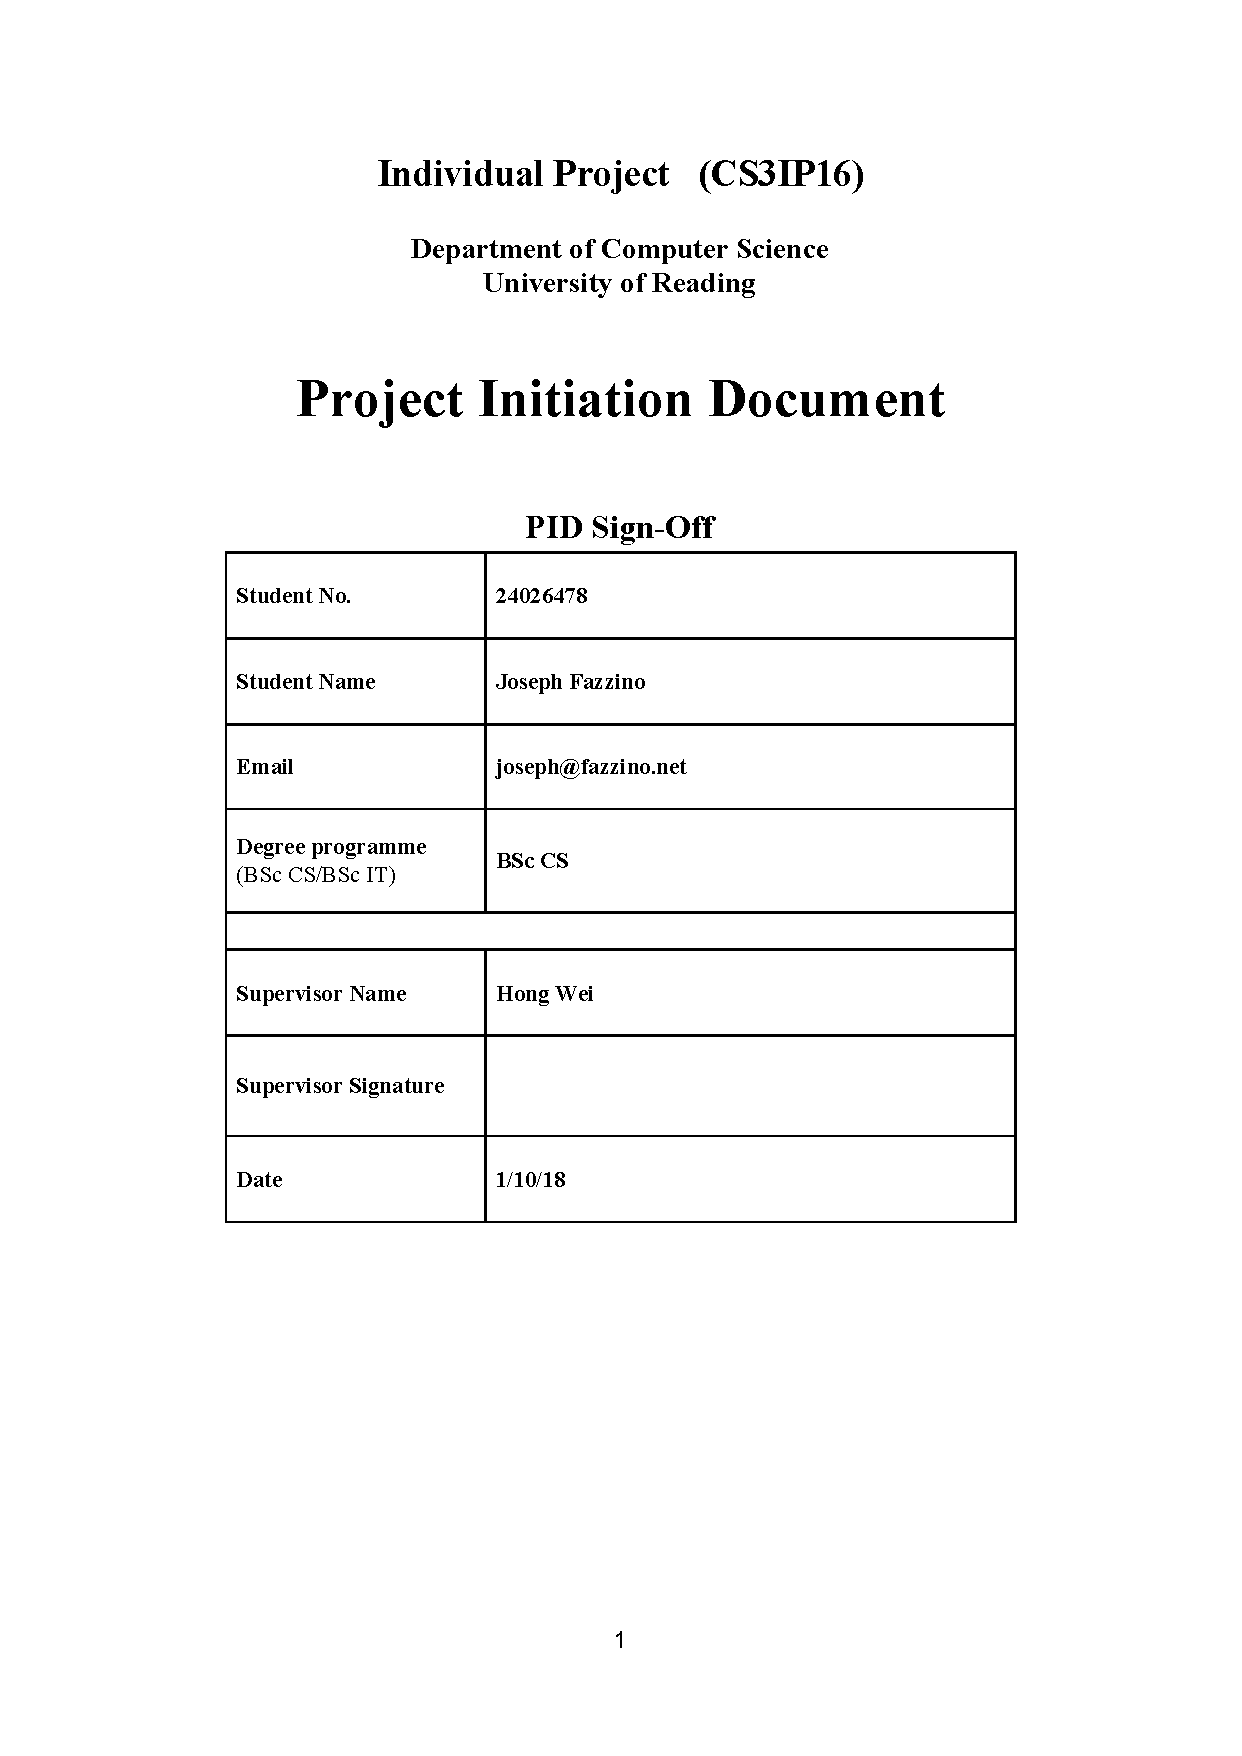
\includepdf[pages=-,pagecommand={},width=\linewidth]{res/PID.pdf}

\chapter{Logbook}
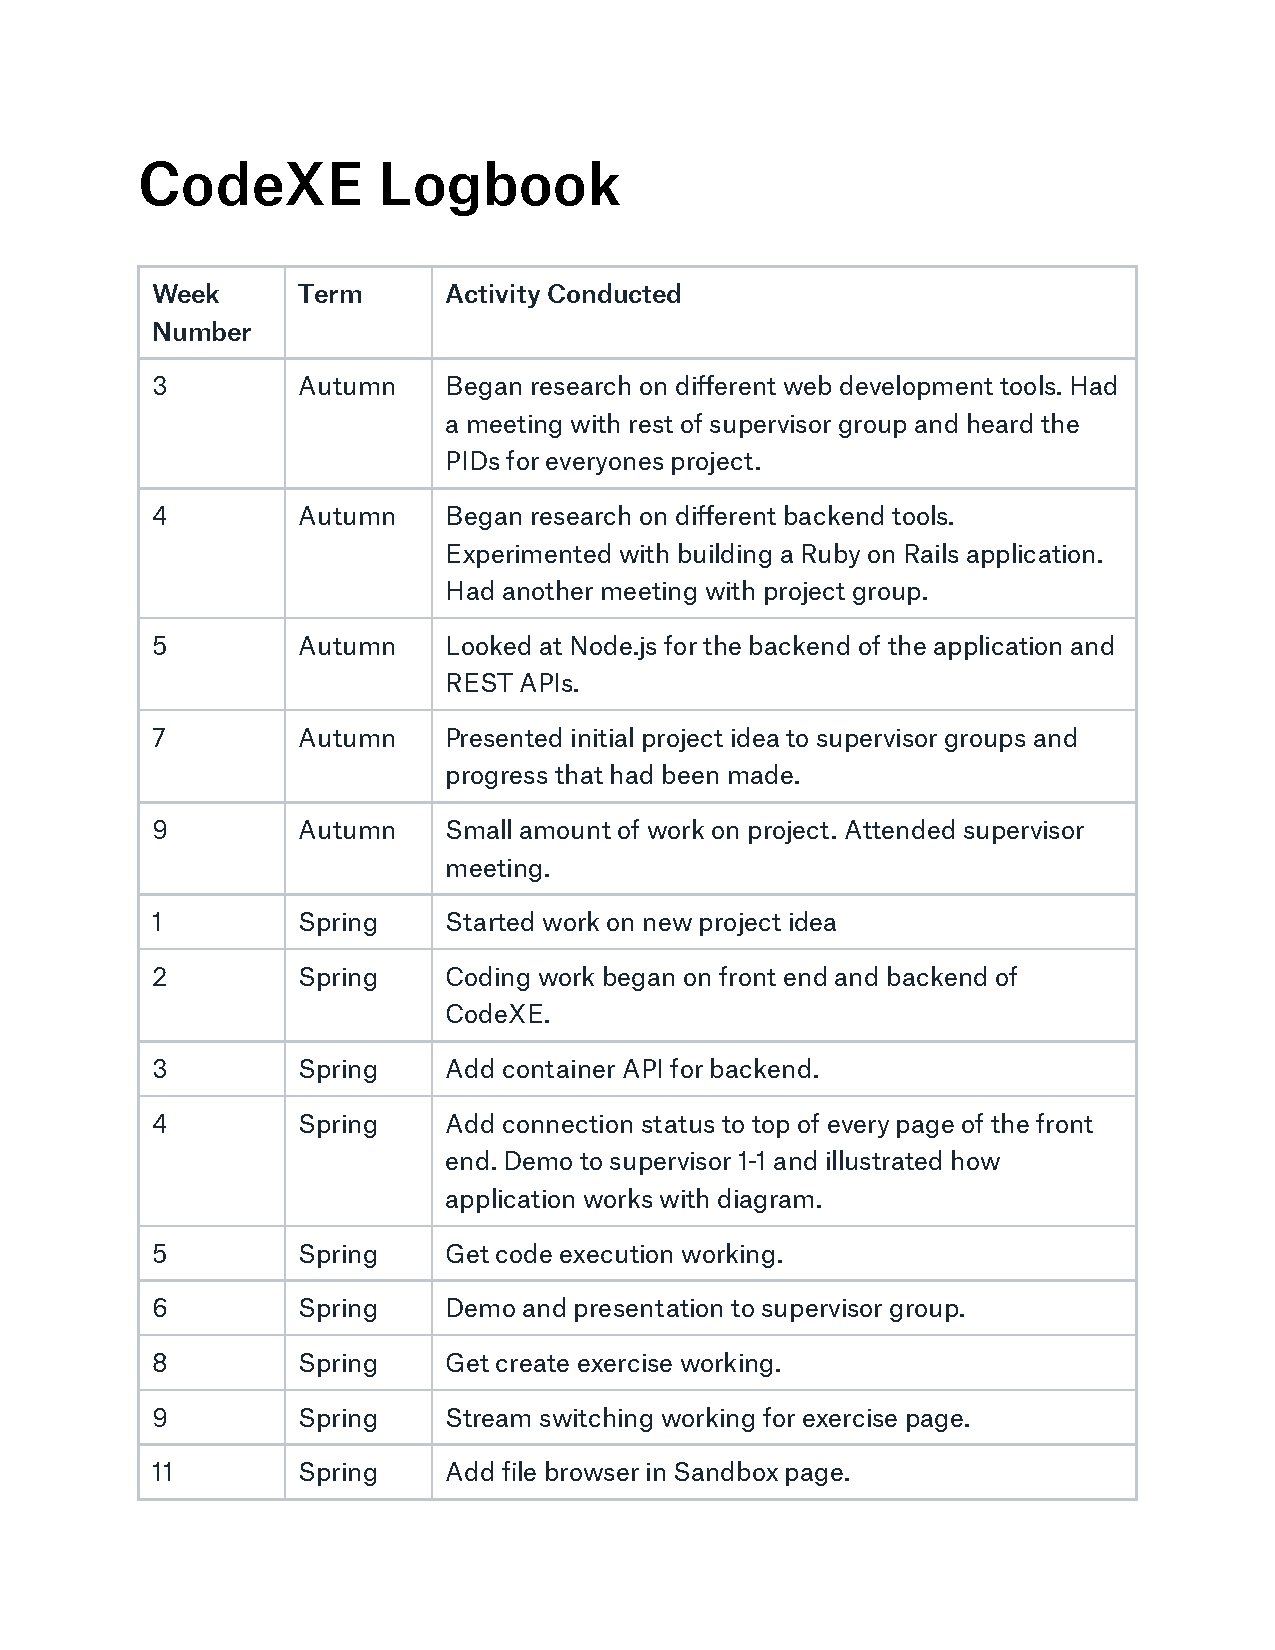
\includepdf[pages=-,pagecommand={},width=\linewidth]{res/CodeXE_Logbook.pdf}

\chapter{Code Repositories}
Front-end - \texttt{https://github.com/joefazz/codexe}\\
Back-end - \texttt{https://github.com/joefazz/Midgard}\\
Ahab - \texttt{https://github.com/joefazz/Ahab}
\end{appendices}



\end{document}
